\begin{figure}[tb]
\centering
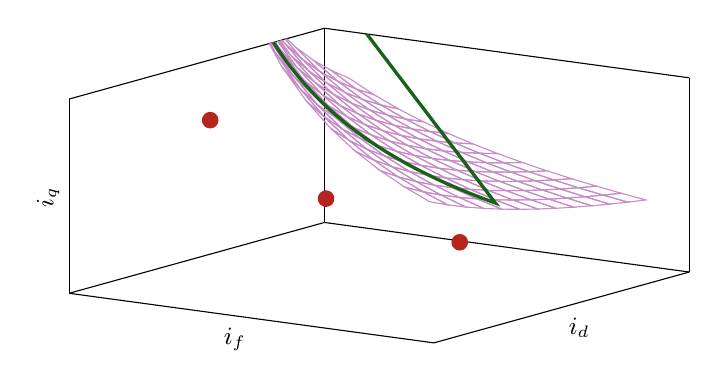
\begin{tikzpicture}[font=\small]
 \begin{axis}[width=.78\linewidth,height=.46\linewidth,view={35}{24},
  xlabel={$i_f$},ylabel={$i_d$},zlabel={$i_q$},ticks=none,
  xmin=0,xmax=2.3,ymin=-.4,ymax=2.2,zmin=0,zmax=2.4]
  \addplot3[mesh,draw=Purple!45,domain=.28:2.15,y domain=-.2:2.0,samples=13,samples y=13]
   ({x},{y},{1.15/(.25*y+.35*x)});
  \addplot3[ForestGreen!70!black,very thick,domain=.35:2.05,samples=80]
   ({x},{.22+.20*x},{1.15/(.25*(.22+.20*x)+.35*x)});
  \addplot3[only marks,mark=*,BrickRed,mark size=2.8pt]
   coordinates {(.45,.31,2.02)(1.1,.44,1.18)(1.85,.59,.79)};
 \end{axis}
\end{tikzpicture}
\caption{Moving optimum manifold.  The translucent surface is a constant
torque set; the dark curve represents the conditional minimum-loss stator
allocation as the slow field current changes.  Fast currents can track this
curve only when time-scale separation and voltage margin are adequate.}
\label{fig:moving-manifold}
\end{figure}

